\section{Структура данных}

В данном наборе данных представлена информация о случаях схода составов с рельс по причине излома боковой рамы вагона

Анализ данных будет проведен при помощи языка программирования Python3. Выбор пал на данный язык по нескольким причинам:
\begin{description}[font=$\bullet$]
\item большое количество модулей для анализа данных;
\item подробная документация как языка, так и его модулей;
\item удобство и простота работы с данными в форматах csv, xlsx;
\item множество встроенных функций и выразительность языка.
\end{description}

Определим размеры выборки:
\mint{python}|print("shape of data frame:", df.shape)|
\mint{text}|> shape of data frame: (56, 12)|

Выведем названия факторов:
\mint{python}|print(df.columns)|
\begin{minted}[fontsize=\footnotesize]{text}
> Index(['Дата', 'Количество вагонов', 'Макс. число вагонов в сходе',
'Общее количество вагонов', 'Количество сшедших вагонов', 'Скорость',
'Вес', 'Загрузка', 'Стрелочный перевод', 'Кривизна', 'Профиль пути',
'Режим движения'],
dtype='object')
\end{minted}

\begin{flushleft}
Получим первые 5 записей из набора:
\end{flushleft}
\begin{table}[H]
\resizebox{\textwidth}{!}{%
    \begin{tabular}{|l|l|p{2.5cm}|p{3cm}|p{3cm}|p{3cm}|l|l|l|p{3cm}|l|p{3cm}|p{3cm}|}
        \hline
        № & Дата & Количество вагонов & Макс. число вагонов в сходе & Общее количество вагонов & Количество сшедших вагонов & Скорость & Вес & Загрузка &
        Стрелочный перевод & Кривизна & Профиль пути & Режим движения \\ \hline
        \textbf{1} & 2013-01-08 & 56.0 & 19.0 & 58.0 & 1  & 57.0 & 3402.0 & 0.547101 & 0 & 0.000000 & 0.0007 & NaN \\ \hline
        \textbf{2} & 2013-01-09 & 60.0 & 25.0 & 62.0 & 1  & 72.0 & 4082.0 & 0.652657 & 0 & 0.000000 & 0.0009 & NaN \\ \hline
        \textbf{3} & 2013-01-10 & 60.0 & 4.0  & 64.0 & 1  & 15.0 & 4420.0 & 0.734300 & 0 & 0.001639 & NaN    & 3.0 \\ \hline
        \textbf{4} & 2013-01-12 & 66.0 & 63.0 & 68.0 & 21 & 67.0 & 5699.0 & 0.918094 & 0 & 0.002326 & 0.0060 & NaN \\ \hline
        \textbf{5} & 2013-01-19 & 67.0 & 34.0 & 69.0 & 1  & 69.0 & 5854.0 & 0.932944 & 0 & 0.000000 & 0.0006 & 2.0 \\ \hline
    \end{tabular}%
}
\captionof{table}{первые 5 записей в наборе данных}
\label{tab:first_5_records}
\end{table}

Получим основные статистики по данным с помощью команды\\
\mintinline{python}|print(df.describe())| (для краткости названия признаков заменены на f1, f2, $\dots$, f11, признак "Дата" не рассматривается).

\begin{table}[H]
\resizebox{\textwidth}{!}{%
    \begin{tabular}{|l|l|l|l|l|l|l|l|l|l|l|l|}
        \hline
        \textbf{} & \textbf{f1} & \textbf{f2} & \textbf{f3} & \textbf{f4} & \textbf{f4} & \textbf{f6} & \textbf{f7} & \textbf{f8} & \textbf{f9} & \textbf{f10} & \textbf{f11} \\ \hline
        \textbf{count} & 54.000000 & 51.000000 & 54.000000 & 56.000000 & 53.000000 & 54.000000 & 54.000000 & 56.000000 & 46.000000 & 44.000000 & 33.000000 \\ \hline
        \textbf{mean} & 63.870370 & 37.137255 & 66.407407 & 3.875000 & 49.150943 & 5126.629630 & 0.817678 & 0.107143 & 0.000806 & -0.000384 & 1.666667 \\ \hline
        \textbf{std} & 9.790342 & 21.543463 & 10.053665 & 6.081455 & 18.450971 & 1438.743887 & 0.243936 & 0.312094 & 0.001171 & 0.005689 & 0.777282 \\ \hline
        \textbf{min} & 24.000000 & 2.000000 & 26.000000 & 1.000000 & 9.000000 & 998.000000 & 0.179710 & 0.000000 & 0.000000 & -0.011500 & 1.000000 \\ \hline
        \textbf{25\%} & 60.000000 & 17.500000 & 62.500000 & 1.000000 & 35.000000 & 4155.500000 & 0.690451 & 0.000000 & 0.000000 & -0.004750 & 1.000000 \\ \hline
        \textbf{50\%} & 66.000000 & 43.000000 & 68.000000 & 1.000000 & 51.000000 & 5722.000000 & 0.925519 & 0.000000 & 0.000000 & 0.000000 & 1.000000 \\ \hline
        \textbf{75\%} & 68.000000 & 56.500000 & 71.750000 & 2.250000 & 64.000000 & 6010.250000 & 0.995586 & 0.000000 & 0.001479 & 0.001875 & 2.000000 \\ \hline
        \textbf{max} & 96.000000 & 72.000000 & 100.000000 & 26.000000 & 78.000000 & 8806.000000 & 1.076087 & 1.000000 & 0.005000 & 0.010900 & 3.000000 \\ \hline
    \end{tabular}%
}
\captionof{table}{основные статистики}
\label{tab:basic_stats}
\end{table}

Заметим, что в данных есть пропуски, так признак "Режим движения" (f11) содержит только 33 записи. Также много пропусков у признаков "Кривизна" (f9) и "Профиль пути" (f10).

Построим матрицу корреляции признаков:
\begin{minted}{python}
corrmat = df.corr()
f, ax = plt.subplots(figsize=(12, 9))
sns.heatmap(corrmat, vmax=.8, square=True)
\end{minted}

\begin{figure}[H]
\begin{center}
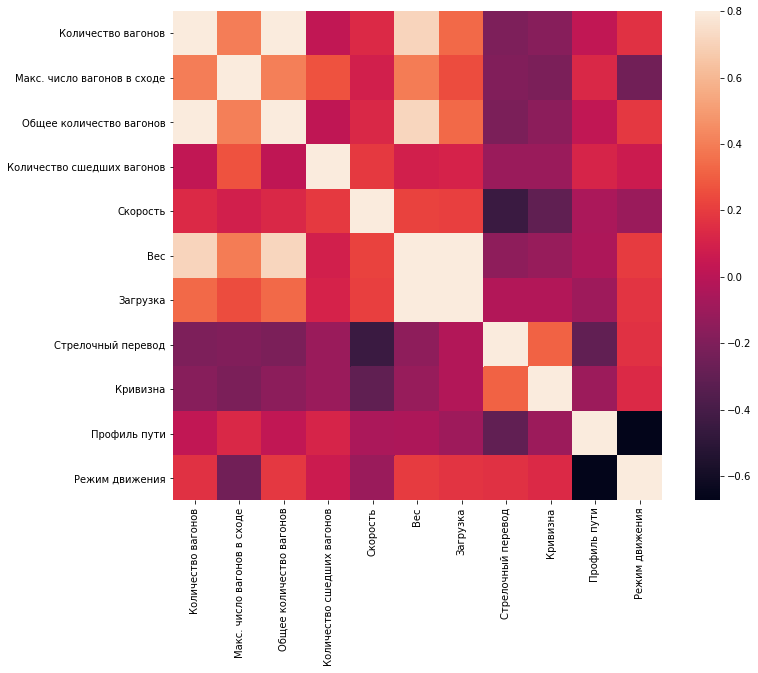
\includegraphics[width=0.6\linewidth]{src/img/df_corr}
\caption{Корреляция признаков}
\label{fig:df_corr}
\end{center}
\end{figure}


Из матрицы видно, что признаки "Количество вогонов" и "Общее число вагонов" имеют сильную корреляцию. Также "Вес" и "Загрузка" сильно коррелируют. Менее сильная корреляция наблюдается у признаков "Вес" и "Общее число вагонов". Также заметим, что у "Профиль пути" и "Режим движения" наблюдается сильная обратная корреляция. Многие зависимости можно нетрудно объяснить: чем больше вагонов в составе, тем больше вес, чем больший вес, тем, как правило, большая загруженность. Таким образом, можно прийти к выводу, что в данные в наборе избыточны, поскольку несколько признаков несут одинаковое количество информации. Поэтому эти зависимости приводят к проблеме мультиколлинеарности, что приведет к эффекту переобучения в линейных моделях. Для решения данной проблемы нужно исключить коррелирующие признаки, и, возможно, добавить новые. Решение проблемы мультиколлинеарности смотри в главе "Линейная регрессия".

\section{Пропуски в данных}

Из таблицы \ref{tab:basic_stats} видно, что в последних четырех признаках присутствуют пропуски в данных.

Существует методы по решению проблемы с пропусками в данных:
\begin{description}[font=$\bullet$]
    \item удалить все записи в которых есть хотя бы одно пустое поле. При использовании этого метода для данного набора данных существует риск того, что оставшегося множества записей не хватит для получения приемлемого качества построенной модели;
    \item заменить пропуски на средние значение по признаку;
    \item заменить пропуски на медианные значение по признаку. В отличие от среднего значения замена на медианное позволяет избежать сильного влияния выбросов на итоговое значение.
\end{description}
При решении задачи будут поочередно использованы все 3 метода борьбы с пропусками, предпочтение будет отдаваться тем моделям, у которых будут более лучшие показатели метрик качества.

\section{Экстремальные значения}

Для поиска выбросов построим графики, изображающие отношения между парами признаков.\\

\begin{figure}[h]
\begin{center}
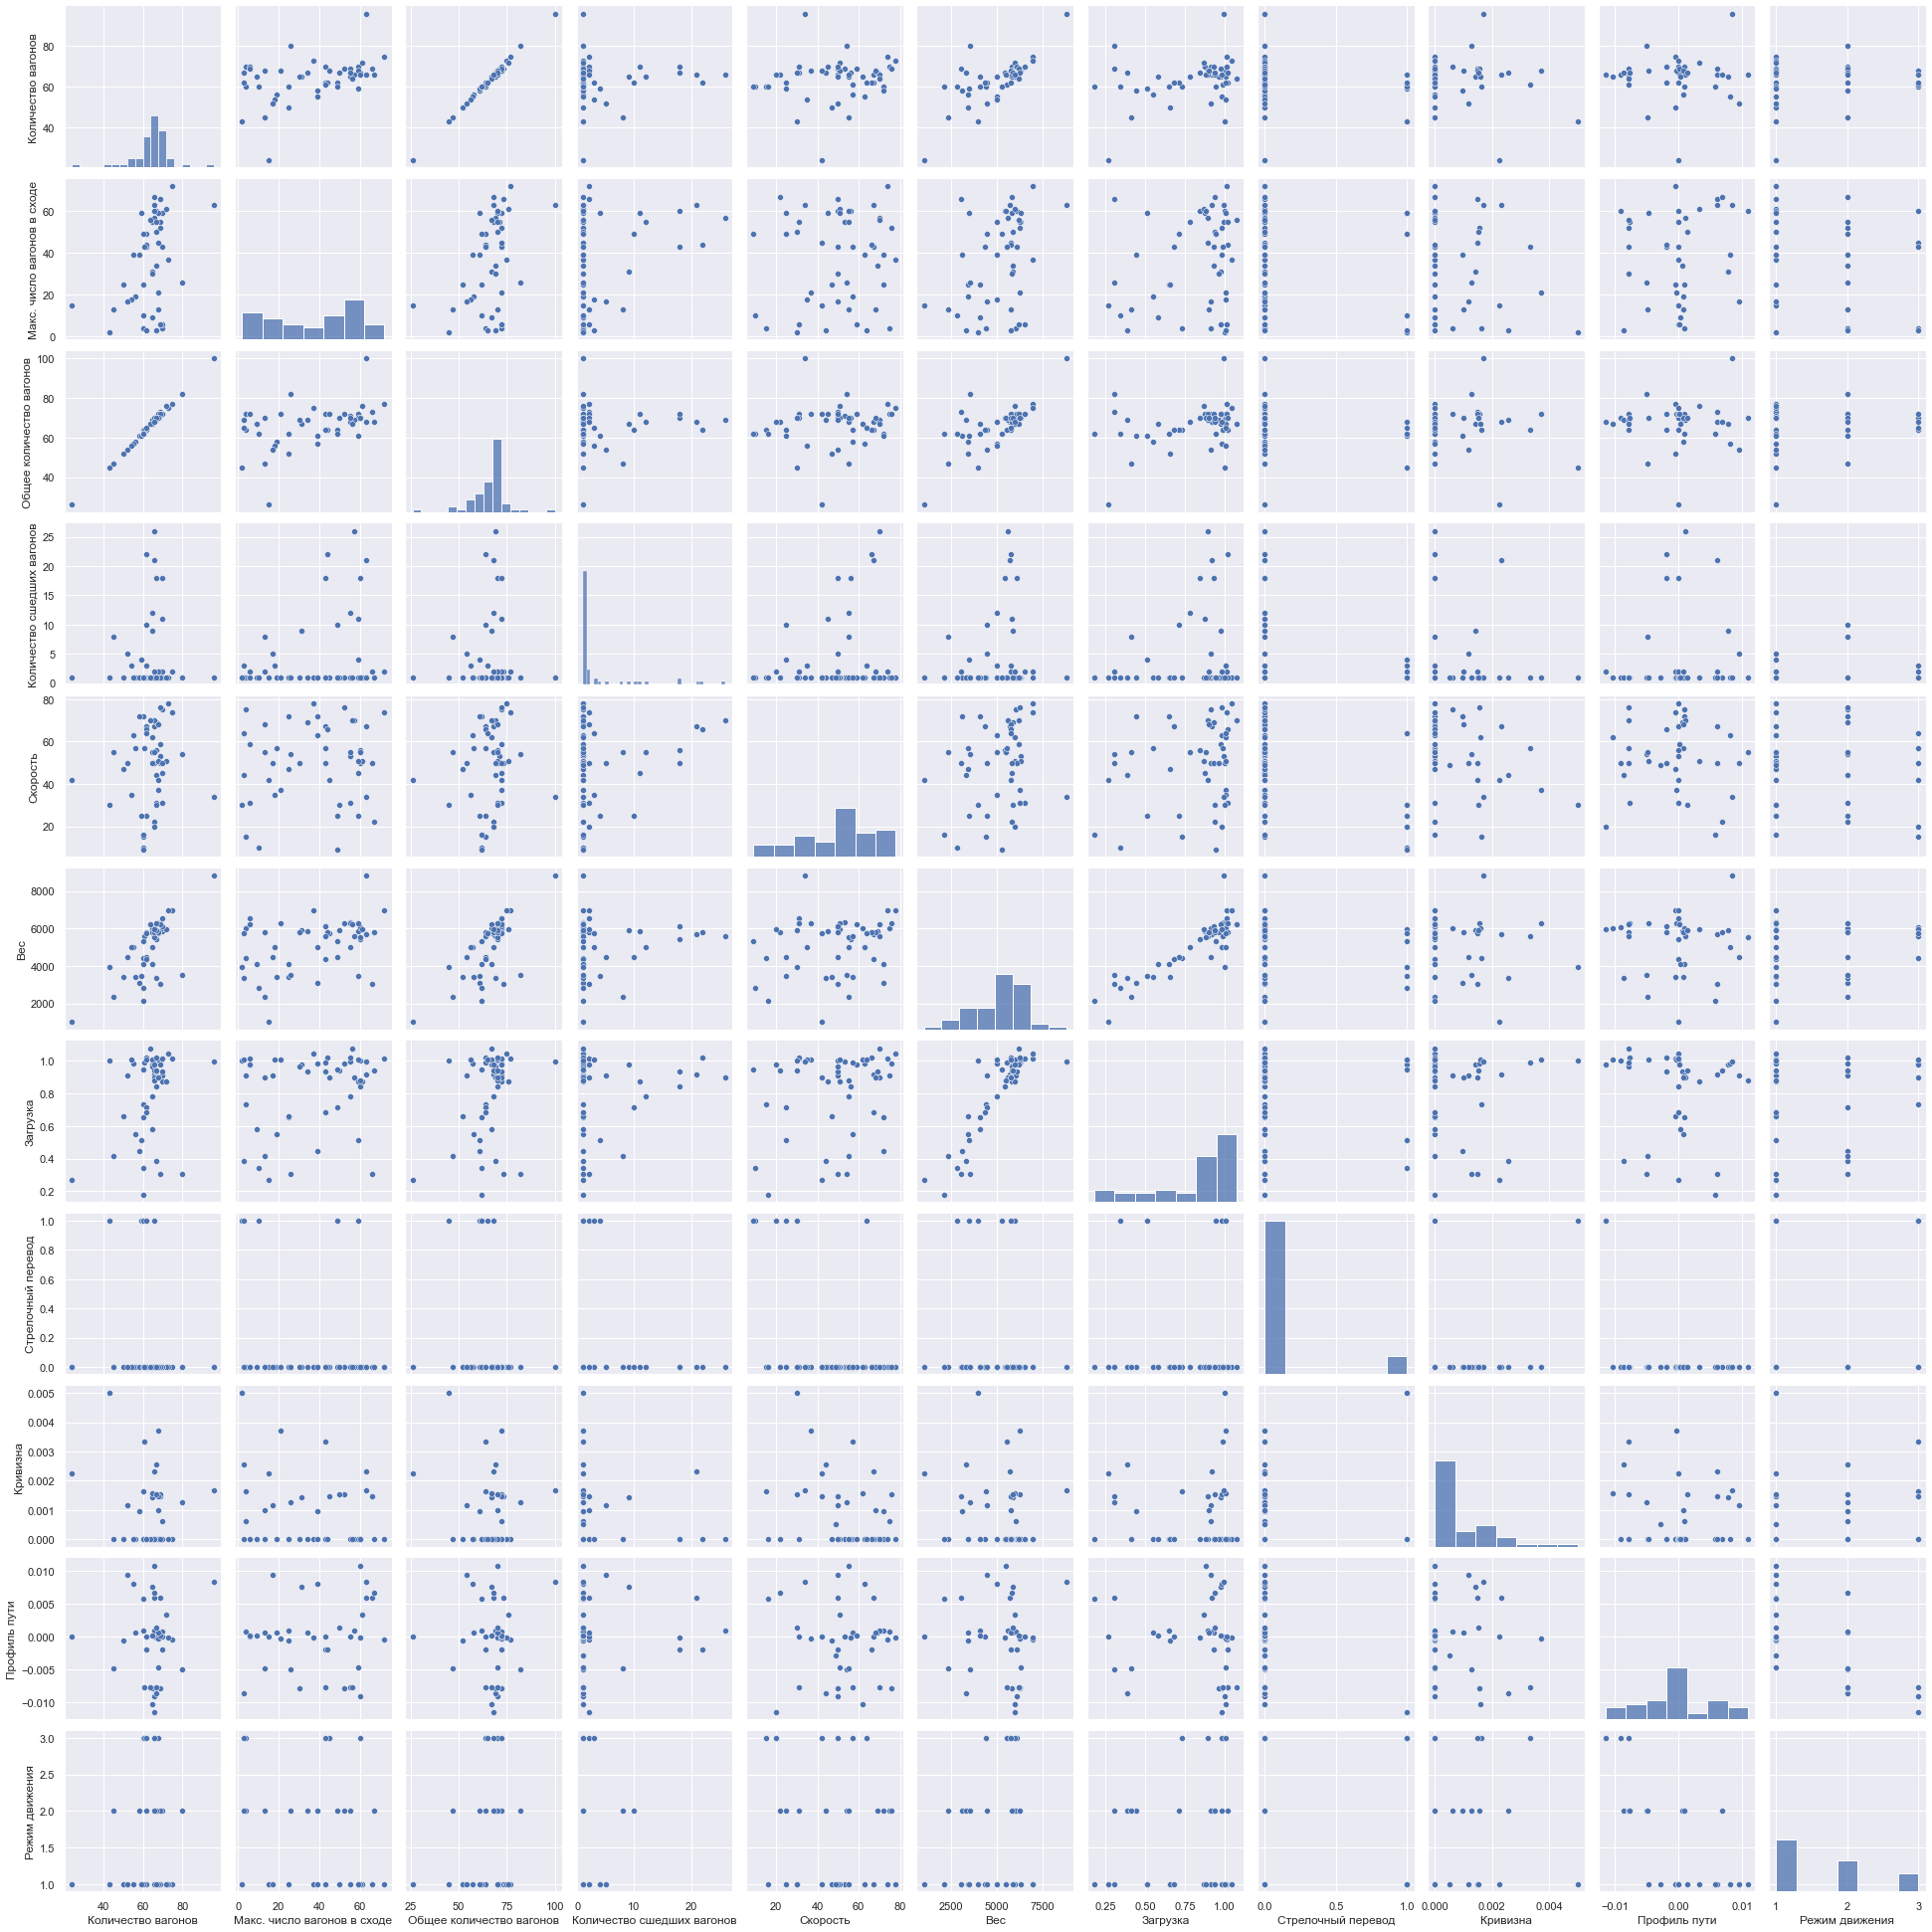
\includegraphics[width=0.9\linewidth]{src/img/pair_plot.png}
\caption{Пары признаков}
\label{fig:pair_plot}
\end{center}
\end{figure}

Изучив таблицу \ref{tab:basic_stats}, а также при детальном рассмотрении графиков \ref{fig:pair_plot} выбросов в данных не обнаружено.

